% A map of pairs q : (X, A) -> (Y, B), with images f(X) and g(X).
% Source: book/tex/homology/excision.tex (§ The excision theorem).
\documentclass[border=2mm]{standalone}
\usepackage{tikz}
\usetikzlibrary{arrows.meta}
\definecolor{heavygreen}{rgb}{0,0.5,0}
\begin{document}
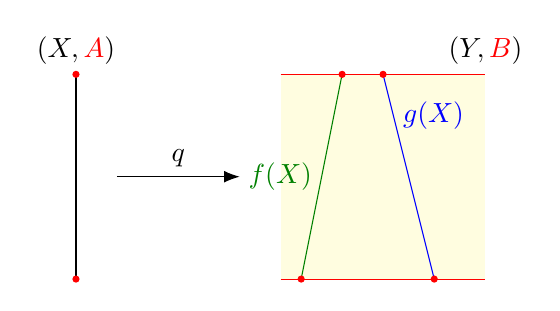
\begin{tikzpicture}[>={Latex[length=2mm]}, scale=2.6]
  \draw (0,0)--(0,1);
  \node[above] at (0,1) {$(X, {\color{red}A})$};
  \fill[red] (0,0) circle (0.5pt); \fill[red] (0,1) circle (0.5pt);
  \draw[->] (0.2,0.5)--(0.8,0.5) node[midway,above] {$q$};
  \fill[yellow!12] (1,0) rectangle (2,1);
  \draw[red] (1,0)--(2,0); \draw[red] (1,1)--(2,1);
  \node[above] at (2,1) {$(Y, {\color{red}B})$};
  \draw[heavygreen] (1.1,0)--(1.3,1) node[midway,left] {$f(X)$};
  \fill[red] (1.1,0) circle (0.5pt); \fill[red] (1.3,1) circle (0.5pt);
  \draw[blue] (1.75,0)--(1.5,1) node[pos=0.8,right] {$g(X)$};
  \fill[red] (1.75,0) circle (0.5pt); \fill[red] (1.5,1) circle (0.5pt);
\end{tikzpicture}
\end{document}
